\section{Experimental Study}
\label{sec:exp}
In this section, we present our experimental findings on
deploying our GCMP detectors to large-scaled real trajectories.
All the experiments are carried out on our in-house cluster: Dianwei. The cluster includes 12 nodes, each of which is equipped with four quad-core 2.2GHz Intel processors, 32 GB memory and gigabit Ethernet. The cluster is installed with CentOS 5.5. operating system.

\textbf{Environment Setup}: We use Yarn\footnote{http://hadoop.apache.org/docs/current/hadoop-yarn/hadoop-yarn-site/YARN.html}
to manage our cluster. One node is dedicated as Yarn's master node, and each other node reserves one core and 2 GB memory for
Yarn processes. We use Apache Spark 1.5.5~\cite{zaharia2012resilient} as the MapReduce framework. Spark takes
the remaining 11 nodes as the computing nodes.
To fully utilize the computing power of the cluster, 
we assign each node to run five executors, each executor takes three cores and 5 GB memory. We use "yarn-cluster" mode
for Spark which randomly picks one executor to act as the Application Master. Such a configuration allows us to run 162 tasks
at the same time. We use HDFS as our storage engine with replicator factor of 1.
The summary of the configuration is as in the following table:


\begin{table} [h]
\centering
\begin{tabular}{|l|c|}
\hline 
Parameter & Value  \\ 
\hline 
Java Version & 1.7.0 \\ 
\hline 
Spark Version & 1.5.5 \\ 
\hline 
spark.driver.memory & 2GB \\ 
\hline 
spark.executor.cores & 3  \\ 
\hline 
spark.executor.instances & 54 \\ 
\hline 
spark.executor.memory & 5GB \\ 
\hline 
spark.master & yarn-cluster \\
\hline 
spark.serializer & KryoSerializer \\ 
\hline 
\end{tabular} 
\end{table}

\textbf{Datasets}: We prepare three real datasets for experiments. The details of the datasets are as follows:
\begin{itemize}
\item{Geolife}~\footnote{http://research.microsoft.com/en-us/projects/geolife/}: this dataset collects 
18,670 trajectories for passengers in Beijing over three years. The data are collected
per around 5 seconds. Each data point records a trajectory ID and the latitude/longitude information.
\item{Shopping}~\footnote{http://www.irc.atr.jp/crest2010\_HRI/ATC\_dataset/}: this dataset contains
 visitors trajectories in ATC shopping center in Osaka. The samples are taken per
 around 0.5 seconds. There are in total 13,183 trajectories. Each data point is a 
 trajectory ID with in-door coordinates.
\item{Taxi}: this dataset records 15,054 Singapore taxi trajectories over one month span. The sample 
rate is around 30 seconds. Each data point is the taxi plate with latitude/longitude information.
\end{itemize}

\textbf{Preprocessing}: We replace timestamps with global sequences for each dataset. The sequence number
$0$ is the earliest timestamp among all trajectories in a dataset. We use the sampling rate of 
each dataset as the tick of the sequence number and every data point is mapped to the nearest ticks. If
several points mapped to the same tick, they are merged by averaging the location coordinates.
For missing data within small intervals (i.e., sequence difference less than 10), 
we use linear interpolation to fill them. 
We then use DBSCAN ($\epsilon=5, minPt=10$ for GeoLife and Shopping, $\epsilon=20, minPt=10$ for Taxi)
as the clustering algorithm for preprocessing.  
Note that both our TRPM and SPARE algorithms treat the preprocessing as a black box and other
spatial clustering methods are also applicable. The clustered snapshots are stored in HDFS in $\langle t, S_t \rangle$ pair, where
$t$ is the timestamp, $S_t$ contains the clusters at snapshot $t$. 
After preprocessing, the statistics of the three datasets are presented in Table~\ref{exp:dataset}. 

\begin{table} [h]
\center
\small
\begin{tabular}{|l|l|l|l|}
\hline
 \textbf{Attributes}& \textbf{ACTShopping} &  \textbf{Geolife} &  \textbf{SingTaxi} \\ 
\hline 
\# objects  & 13,183 & 18,670 & 15,054\\ 
\hline
\# average ts & 3,114  & 2,924 & 19,667 \\ 
\hline
\# data points  & 41,052,242 & 54,594,696 & 296,075,837\\ 
\hline
\# snapshots  & 16,931 & 10,699 & 44,364\\ 
\hline
\# clusters  & 211,403  & 206,704& 536,804\\
\hline
avg. cluster size  & 171 & 223 & 484\\
\hline
%\# of patterns & 3,741 & 4,369  & 7,585 \\
%\hline
\end{tabular}
\caption{Statistics of data set}
\label{exp:dataset}
\end{table}

\textbf{Parameters}: To systematically study the performance of
our algorithms, we conduct experiments on various conditions. The variables
to be tested and their value ranges are listed in Table~\ref{tbl:parameters}. 
Default values are highlighted in bold.
\begin{table}[h]
\small
\begin{tabular}{c|l|l}
\hline 
\textbf{Variables} & \textbf{Meaning} & \textbf{Values} \\ 
\hline 
M & min size of object set &  5, 10,  \textbf{15}, 20, 25 \\ 
\hline 
K & min duration & 120, 150, \textbf{180}, 210, 240 \\ 
\hline 
L & min local duration & 10, 20, \textbf{30}, 40,50 \\ 
\hline 
G & max gap & 10, 15, \textbf{20}, 25, 30 \\ 
\hline
N & number of executors & 1, 14, 24, 34, 44, \textbf{54}\\ 
\hline 
\end{tabular} 
\caption{Variables and their default values}
\label{tbl:parameters}
\end{table}

\textbf{Number of patterns under different parameters}: We first 
analyze the number of patterns exist in each dataset under different conditions. The results are presented in Figures~\ref{exp:patterns_vary}. As expected, the number of patterns differs under in different scenarios. Larger $M$, $L$, $K$ imply smaller number of patterns, because lesser patterns are able to meet stricter $M$, $L$, $K$ constraints. In contrast, larger $G$ implies larger number of patterns. This is because larger gaps relaxes the pattern constraint. Two interesting observations are made on $L$ and $G$.
First, as $L$ increases from $10$ to $20$, the number of patterns drops quickly (50\% less). Second, opposed to $L$'s trend, as $G$ reaches to $30$ from $25$, the number of patterns bursts (near 50\% more). The distribution of patterns under $G$ and $L$ reveals that there are many companions in real life which are short and intermittent. With GCMP, we can discover these patterns by adjusting property $L$ and $G$s.


\begin{figure}[h]
\centering
 	 \begin{subfigure}[b]{0.23\textwidth}
        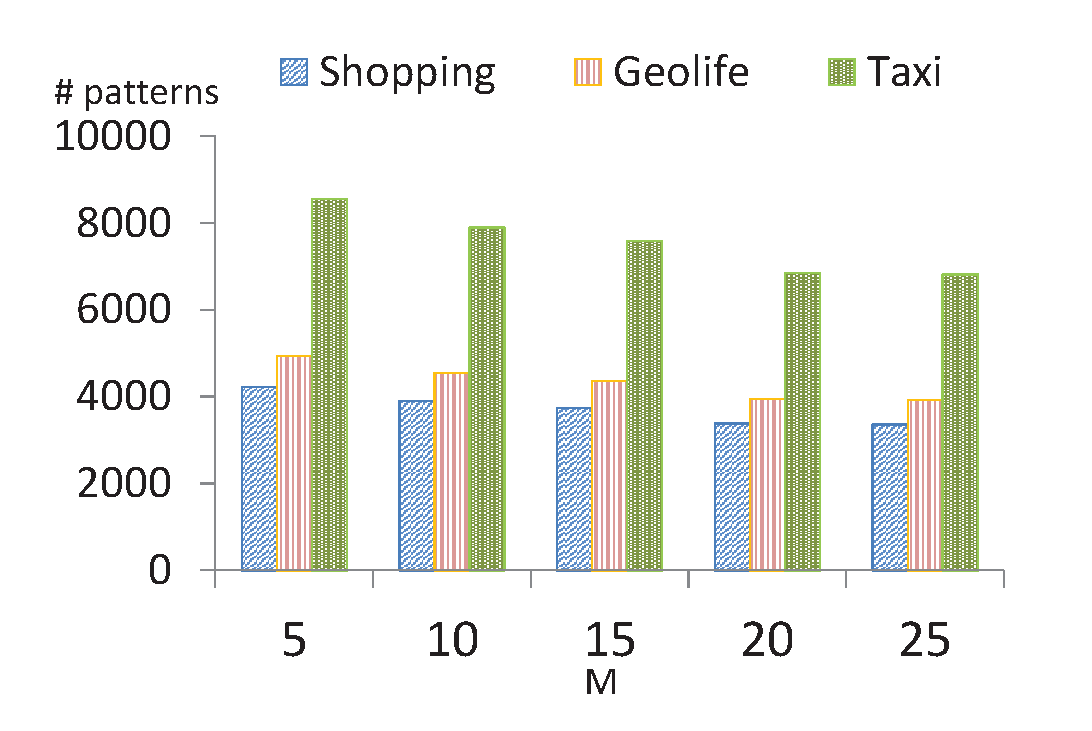
\includegraphics[width=\textwidth]{/exp/effectiveness/patterns_vary_M.eps}
        \caption{Number of patterns vary $M$}
    \end{subfigure}
    \begin{subfigure}[b]{0.23\textwidth}
        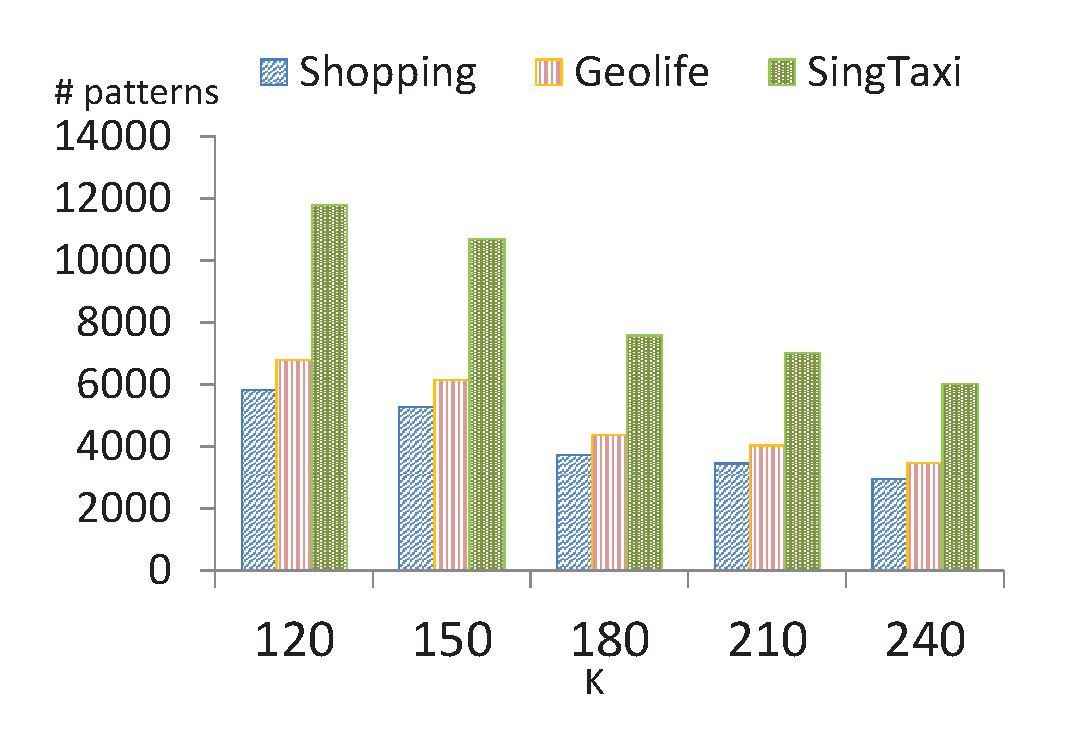
\includegraphics[width=\textwidth]{/exp/effectiveness/patterns_vary_K.eps}
        \caption{Number of patterns vary $K$}
    \end{subfigure}  
    \begin{subfigure}[b]{0.23\textwidth}
        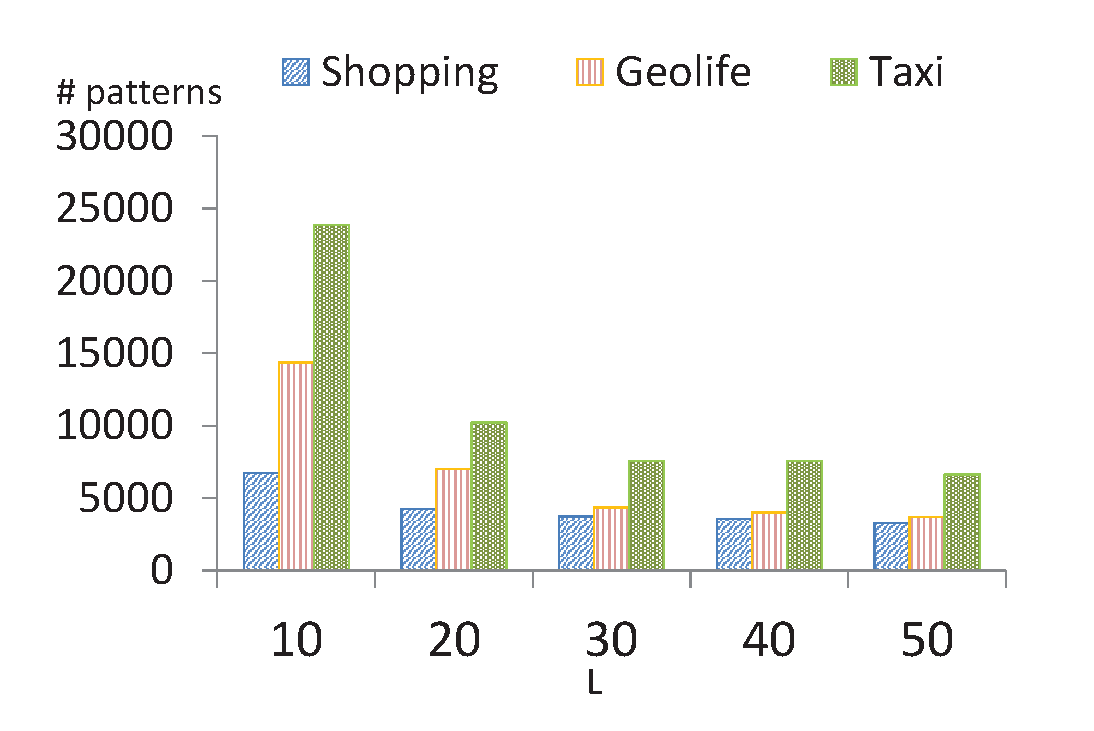
\includegraphics[width=\textwidth]{/exp/effectiveness/patterns_vary_L.eps}
        \caption{Number of patterns vary $L$}
    \end{subfigure}
    \begin{subfigure}[b]{0.23\textwidth}
        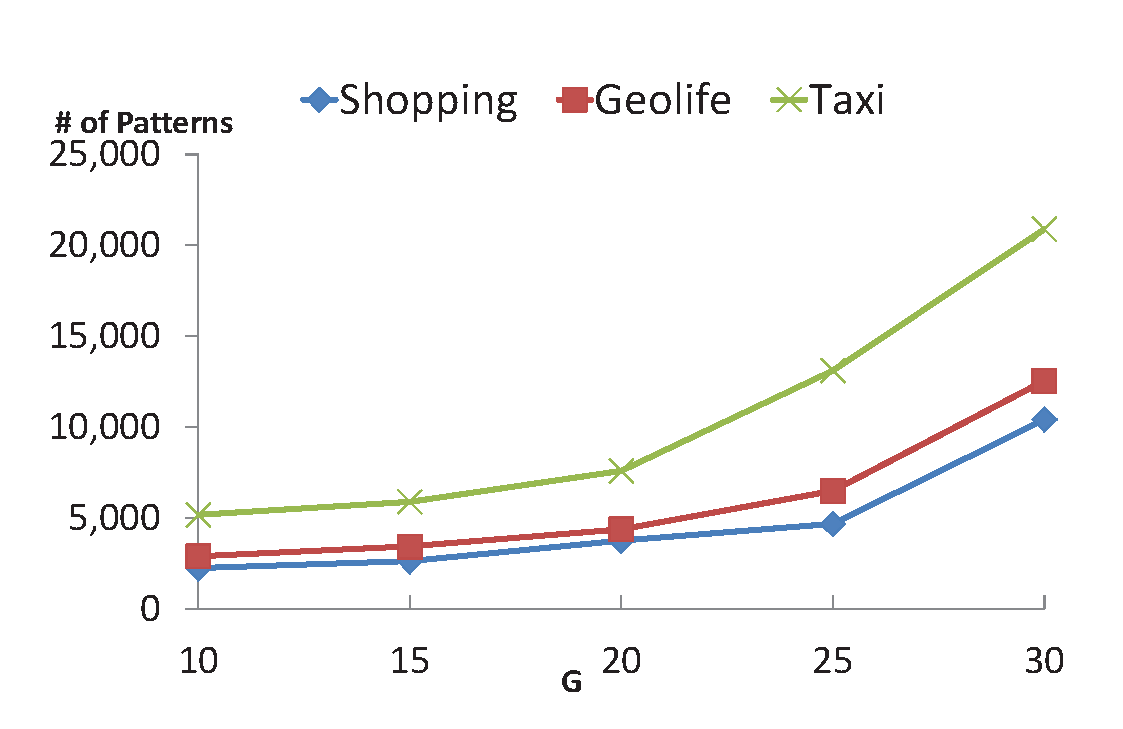
\includegraphics[width=\textwidth]{/exp/effectiveness/patterns_vary_G.eps}
        \caption{Number of patterns vary $G$}
    \end{subfigure}    
\caption{Number of patterns discovered from real datasets}
\label{exp:patterns_vary}
\end{figure}


\textbf{Algorithms}: We implement TRPM, SPARE and SPARE-LB for comparison study. TRPM and SPARE are implement as described in Section 4 and 5. SPARE-LB extends SPARE by appending an additional load balance stage to the map phase. 
When the mappers complete, SPARE-LB collects the size of stars from all mappers. 
Then a best-fit strategy is applied for task allocation. In best-fit, 
tasks are assigned in decreasing order of their sizes, and the most costly
unassigned task is allocated to the current mostly empty reducer. 
In SPARE-LB, we simply use the number of edges in stars as a cost estimation. The other
part of SPARE-LB is identical with SPARE.





%\subsection{Effects of $G$ on GCMP}
%\begin{figure*}[t]
%\centering
%    \begin{subfigure}[b]{0.3\textwidth}
%        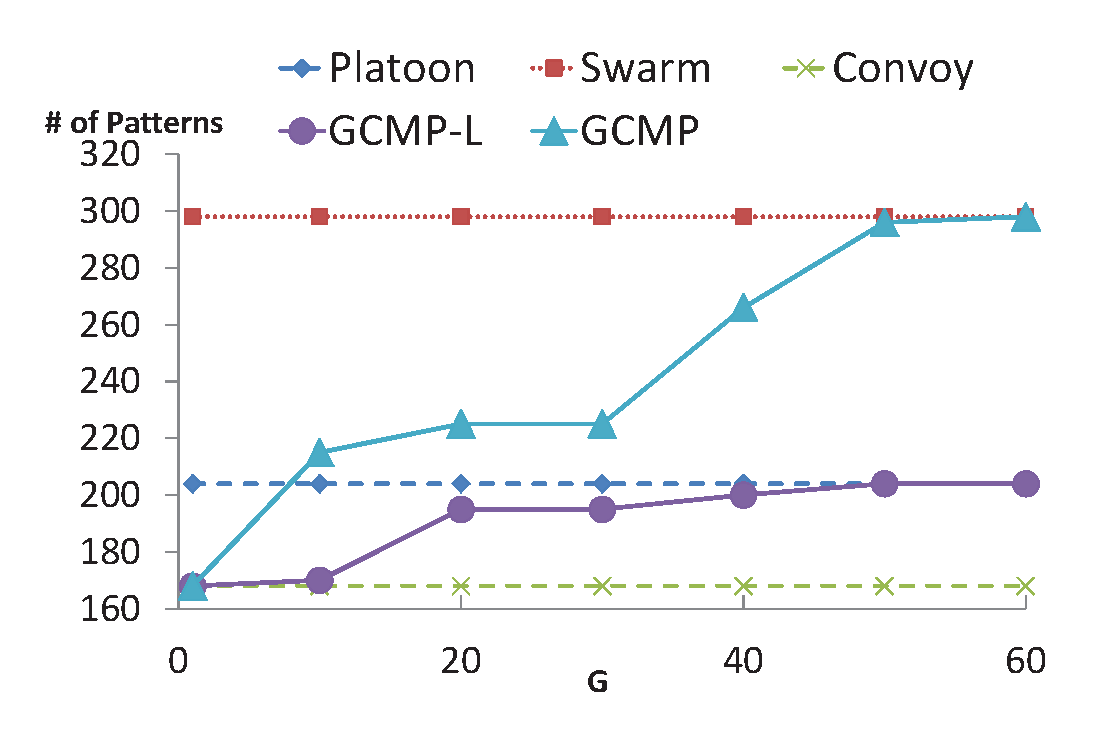
\includegraphics[width=\textwidth]{exp/effectiveness/effect_geolife.eps}
%        \caption{Geolife}
%    \end{subfigure}
%    \begin{subfigure}[b]{0.33\textwidth}
%        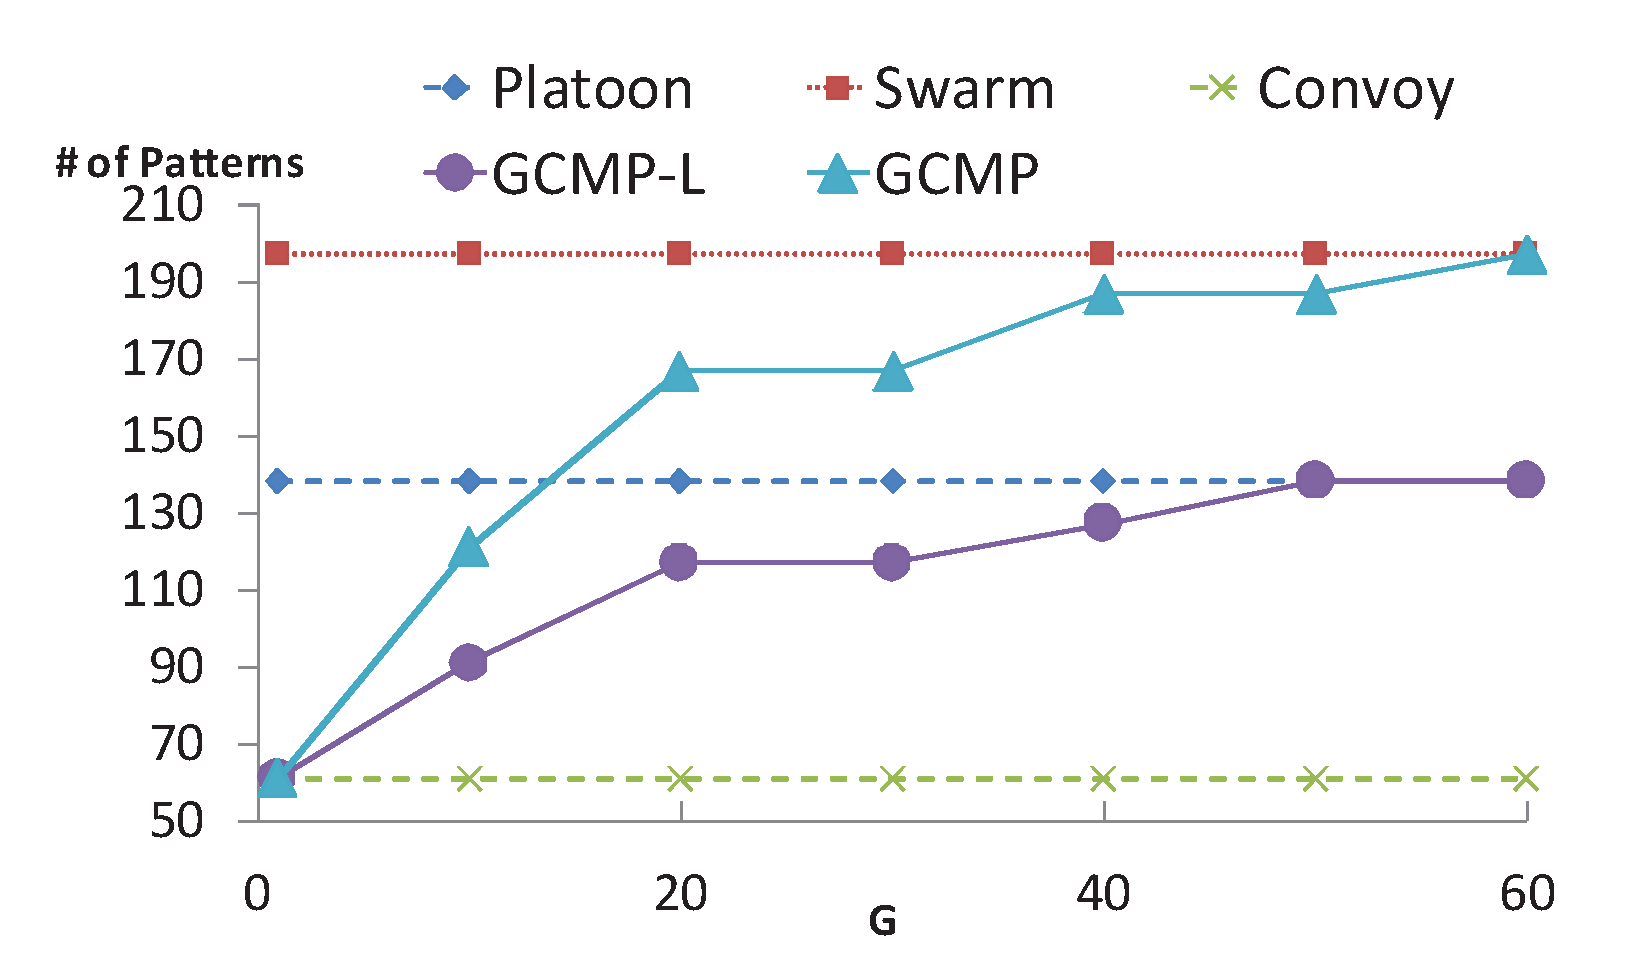
\includegraphics[width=\textwidth]{exp/effectiveness/effect_shopping.eps}
%        \caption{ACTShopping}
%    \end{subfigure}
%    \begin{subfigure}[b]{0.3\textwidth}
%        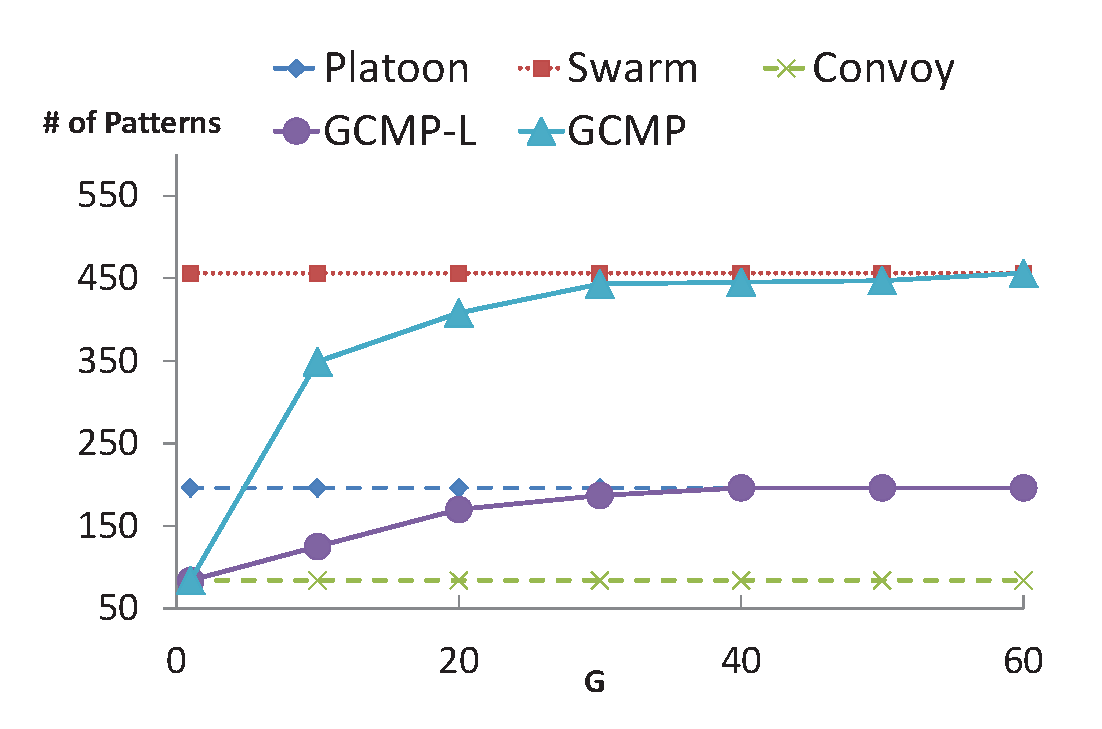
\includegraphics[width=\textwidth]{exp/effectiveness/effect_taxi.eps}
%        \caption{SingTaxi}
%    \end{subfigure}
%\caption{Effectiveness of GCMP model on sampled datasets.}
%\label{exp:effectiveness}
%\end{figure*}
%We first study the effects of introducing gap parameter $G$ on pattern discovery.
%As shown in Figure~\ref{fig:related_work_scalability},
%existing works are not able to handle large trajectories, 
%we sample and cluster $1$ million trajectory points from the three real data.
%We use two instances of GCMPs, GCMP-L where the $L$ value is default and GCMP where $L = 1$.  We measure the number
%of patterns discvoered by different methods. The results are presented in Figure~\ref{exp:effectiveness}.
%
%We can see from Figures~\ref{exp:effectiveness} that the number of patterns
%discovered by GCMP is positively related to $G$. When $G =1$, the number
%of patterns returned by GCMP and GCMP-L are identical to \emph{convoy}. As $G$ grows,
%the number returned by GCMP-L converges to \emph{platoon}. For example, in (a), two
%patterns converge when $G$ is $40$. Similarly in (b) and (c), two patterns converge
%when $G$ is $50$. The reason is that when $G$ is large enough,
% all \emph{platoon}s are $G$-connected. Similar
% trend applies between GCMP and \emph{swarm}. As see from the figures, in (a), two
% patterns converge at $G=50$; while in (b) and (c) the two patterns converge
% at $G=60$ and $G=40$ respectively. We further
% note that, existing patterns has different granularity in temporal domain. As we seen
% from the three figures, the number of \emph{swarm} is greater than \emph{platoon} and
% \emph{convoy}. Despite none of the existing patterns are able to fine-grain control
% the temporal domain of patterns, GCMP can discover the patterns more precisely. 
% These results confirms the usefulness of GCMP in expressing other patterns.
%  
%


\subsection{Performance Comparison}
Since the both TRPM and SPARE utilizes pruning rules that related to the pattern parameters $M$,$K$,$L$,$G$. It is interesting to
see their performances under different settings.
We run the three algorithms using all three datasets 
and report their overall performances in Figures~\ref{exp:performance_vary}.
In brief, all of the three algorithms 
are able to handle the large-scaled real
datasets. However, SPARE algorithms are obviously more efficient than TRPM. 
In the case when $G$ is large (i.e., $G=30$), 
TRMP takes near three hours for Taxi dataset, which is 15 times slower than SPARE algorithms. Besides, SPARE-LB is consistently more efficient than SPARE, with an average of 20\% improvements.
Another general observation
is that all of the three algorithms run slower in the Taxi dataset as compared to
other two datasets. This is because Taxi dataset contains
the most number of temporal data points, which is around 7 times of Shopping
dataset and 5 times of geolife dataset.
 In summary, SPARE outperforms TRMP in all cases. Next, we analyze the details of each experiments.

\begin{figure*}[t]
\centering
    \begin{subfigure}[b]{0.23\textwidth}
        \includegraphics[width=\textwidth]{/exp/performance/shopping_vary_M.eps}
        \caption{Shopping vary $M$}
    \end{subfigure}
    \begin{subfigure}[b]{0.23\textwidth}
        \includegraphics[width=\textwidth]{/exp/performance/shopping_vary_K.eps}
        \caption{Shopping vary $K$}
    \end{subfigure}
    \begin{subfigure}[b]{0.23\textwidth}
        \includegraphics[width=\textwidth]{/exp/performance/shopping_vary_L.eps}
        \caption{Shopping vary $L$}
    \end{subfigure}
       \begin{subfigure}[b]{0.23\textwidth}
        \includegraphics[width=\textwidth]{/exp/performance/shopping_vary_G.eps}
        \caption{Shopping vary $G$}
    \end{subfigure}

	\begin{subfigure}[b]{0.23\textwidth}
        \includegraphics[width=\textwidth]{/exp/performance/geolife_vary_M.eps}
        \caption{Geolife vary $M$}
    \end{subfigure}
    \begin{subfigure}[b]{0.23\textwidth}
        \includegraphics[width=\textwidth]{/exp/performance/geolife_vary_K.eps}
        \caption{Geolife vary $K$}
    \end{subfigure}
    \begin{subfigure}[b]{0.23\textwidth}
        \includegraphics[width=\textwidth]{/exp/performance/geolife_vary_L.eps}
        \caption{Geolife vary $L$}
    \end{subfigure}
       \begin{subfigure}[b]{0.23\textwidth}
        \includegraphics[width=\textwidth]{/exp/performance/geolife_vary_G.eps}
        \caption{Geolife vary $G$}
    \end{subfigure}
    
    \begin{subfigure}[b]{0.23\textwidth}
        \includegraphics[width=\textwidth]{/exp/performance/taxi_vary_M.eps}
        \caption{Taxi vary $M$}
    \end{subfigure}
    \begin{subfigure}[b]{0.23\textwidth}
        \includegraphics[width=\textwidth]{/exp/performance/taxi_vary_K.eps}
        \caption{Taxi vary $K$}
    \end{subfigure}
    \begin{subfigure}[b]{0.23\textwidth}
        \includegraphics[width=\textwidth]{/exp/performance/taxi_vary_L.eps}
        \caption{Taxi vary $L$}
    \end{subfigure}
       \begin{subfigure}[b]{0.23\textwidth}
        \includegraphics[width=\textwidth]{/exp/performance/taxi_vary_G.eps}
        \caption{Taxi vary $G$}
    \end{subfigure}       
\caption{Performance of SPARE and TRPM on real datasets under different pattern parameters.}
\label{exp:performance_vary}
\end{figure*}
%\subsubsection{Effects of pattern parameters M,L,K,G}
\textbf{Vary $M$}: Figures~\ref{exp:performance_vary} (a),(e),(i)
present the performance when $M$ changes.
As the figures show, SPARE based algorithms runs much faster than TRPM. We can see that SPARE
speeds up TRPM 2.7 times in Shopping data, 3.1 times in Geolife data and
7 times in Taxi data. An interesting observation is that, the running times
of all algorithms slightly decrease as $M$ grows. This is
because when $M$ becomes bigger, smaller clusters or stars can be directly pruned, which brings in the efficiency.

\textbf{Vary $K$}: Figure~\ref{exp:performance_vary} (b),(f),(j) 
presents the performances when $K$ changes. 
There are two interesting findings. 
First, SPARE based algorithms and TRPM takes different trends as $K$ increases. 
When $K$ increases, SPARE and SPARE-LB tends to run faster
while TRPM continuously slows down. For SPARE, the trends are resulted from more pruning powers brought
by $K$. When $K$ increases, more sequences can be pruned by the \emph{sequence simplification}.
Conversely, TRPM fails to utilize $K$ for pruning. Moreover, as $K$ increases, $\eta$ in TRPM grows, indicating more replication of snapshots. 
This explains the low performance of TRPM.  Second, when $K$ is small (i.e, $K$=120), TRPM could outperform SPARE. This is because smaller $K$ indicates small partition size in TRPM but restricted the pruning power in SPARE. As a result, TRPM wins 10\% in Geolife dataset. However, by leveraging the load balancing, SPARE-LB is still faster than TRPM.

\textbf{Vary $L$}: Figures~\ref{exp:performance_vary} (c)(g)(k) presents the performances when $L$ changes. We can see that SPARE based algorithms are still superior than TRPM, where SPARE-LB outperforms TRPM near 10 times when $L =10$.
An interesting observation is that $L$
provides good pruning power from $10$ to $20$ for both TRPM and SPARE based algorithms. The major reason is that the decrease of $L$ invalidates many candidates (as shown in Figure~\ref{exp:patterns_vary} (c)), thus the prunings in both SPARE and TRPM become more significant.  As $L$ continues to increase, we can see that TRPM's performance gain is larger than SPARE based algorithms. This is because larger $L$ indicates smaller $\eta$, which is more beneficial to TRPM.

\textbf{Vary $G$}: Figures~\ref{exp:performance_vary} (d)(h)(l) presents the performances when $G$ changes.  Unlike other cases, when $G$ increases, both TRPM and SPARE based algorithms run slower. The reason is that large $G$ relaxes the constraint of a pattern, thus the pruning powers of TRPM and SPARE is more restricted. We observe that there is a burst in performance of TRPM when $G$ reach to $30$. The major reason is that when $G$ becomes to 30, the number of valid patterns almost doubles as shown in Figure~\ref{exp:patterns_vary} (d). This indicate that during TRPM's line sweep, very few patterns can be pruned, making the candidate set grows exponentially. Similarly, SPARE algorithms are also affected by the increase of $G$. However we do not observe such a burst for SPARE. The reason is bi-folded. First, SPARE can utilize $K$, $L$ to retain the power of pruning. Second, SPARE leverages \emph{forward closure check} to quickly output valid patterns and avoids to enumerating many candidates.
%
%
% However, since SPARE algorithms are able to utilize $K$, $L$, $M$ in pruning, the 
%
%
%In general, both TRPM and SPARE
%runs slower when $G$ increases. This is because, when $G$ increases, exponentially more valid patterns
%exist. In other words, the pruning powers in TRPM and SPARE become weaker. We notice
%that there is an burst of TRPM as $G$ increases. The major reason is that 
%during line-sweep, if $G$-increases, each candidate needs to wait for more time before expiring.
%This makes the candidate set exponentially grows and 
%the join operation becomes very expensive.
%Unlike TRPM, SPARE is although affected by the increase of $G$, 
%but the impact is marginal as compared
%to TRPM. This is because, although true patterns may become 
%exponentially large as $G$ increases, the \emph{forward closure check} of SPARE
%can quickly output true patterns without enumerating every of its subset.
%\subsubsection{Effects of clusters $\epsilon$, minPt}





%\subsubsection{Anatomy of SPARE and TRPM}



\subsection{Analysis of SPARE and SPARE-LB}
As SPARE based algorithms are superior than TRPM,
we further analyze several more aspects of SPARE namely, \emph{power of pruning}, \emph{load balance} and \emph{scalability}.

\subsubsection{Power of sequence simplification}
One of the core techniques used in SPARE is the \emph{sequence simplification} (see Section 5.2.1). 
As shown in  Algorithm~\ref{algo:apriori_mining}, we use $\mathtt{sim}(T)$
to prune false candidates. To study the power of sequence simplification,
we collect the total number of pairs that are pruned before apriori enumeration. The
statistics are shown in Table~\ref{tbl:pruning} under default parameters. The result states that the \emph{sequence simplification} is a very powerful pruning technique. It cuts off near 90\% of the initial pairs, which significantly reduces the costs
of later enumerations. This confirms the necessity and usefulness of design such a technique.


\begin{table}[h]
\begin{tabular}{|l|c|c|c|}
\hline 
\textbf{Data Set} & \textbf{Shopping} & \textbf{Geolife} & \textbf{Taxi} \\ 
\hline 
Before pruning & 878,309 &  1,134,228 & 2,210,101 \\ 
\hline 
After pruning & 76,672 & 123,410 & 270,921 \\ 
\hline 
Prune ratio & 91.2\% & 89.1\% & 87.7\% \\ 
\hline 
\end{tabular} 
%
%\begin{tabular}{|c|c|c|c|}
%\hline 
%\textbf{Dataset} & \textbf{Initial Candidates} & \textbf{Real Candidates} & \textbf{Prune-Ratio} \\ 
%\hline 
%Shopping & 878,309 & 76,672 &  91.2\%\\ 
%\hline 
%Geolife & 1,134,228 & 123,410 & 89.1\% \\ 
%\hline 
%Taxi & 2,210,101 & 270.921 & 87.7\% \\ 
%\hline 
%\end{tabular} 
\caption{Pruning power of SPARE}
\label{tbl:pruning}
\end{table}

\begin{figure}[h]
\centering
	\begin{subfigure}[b]{0.22\textwidth}
        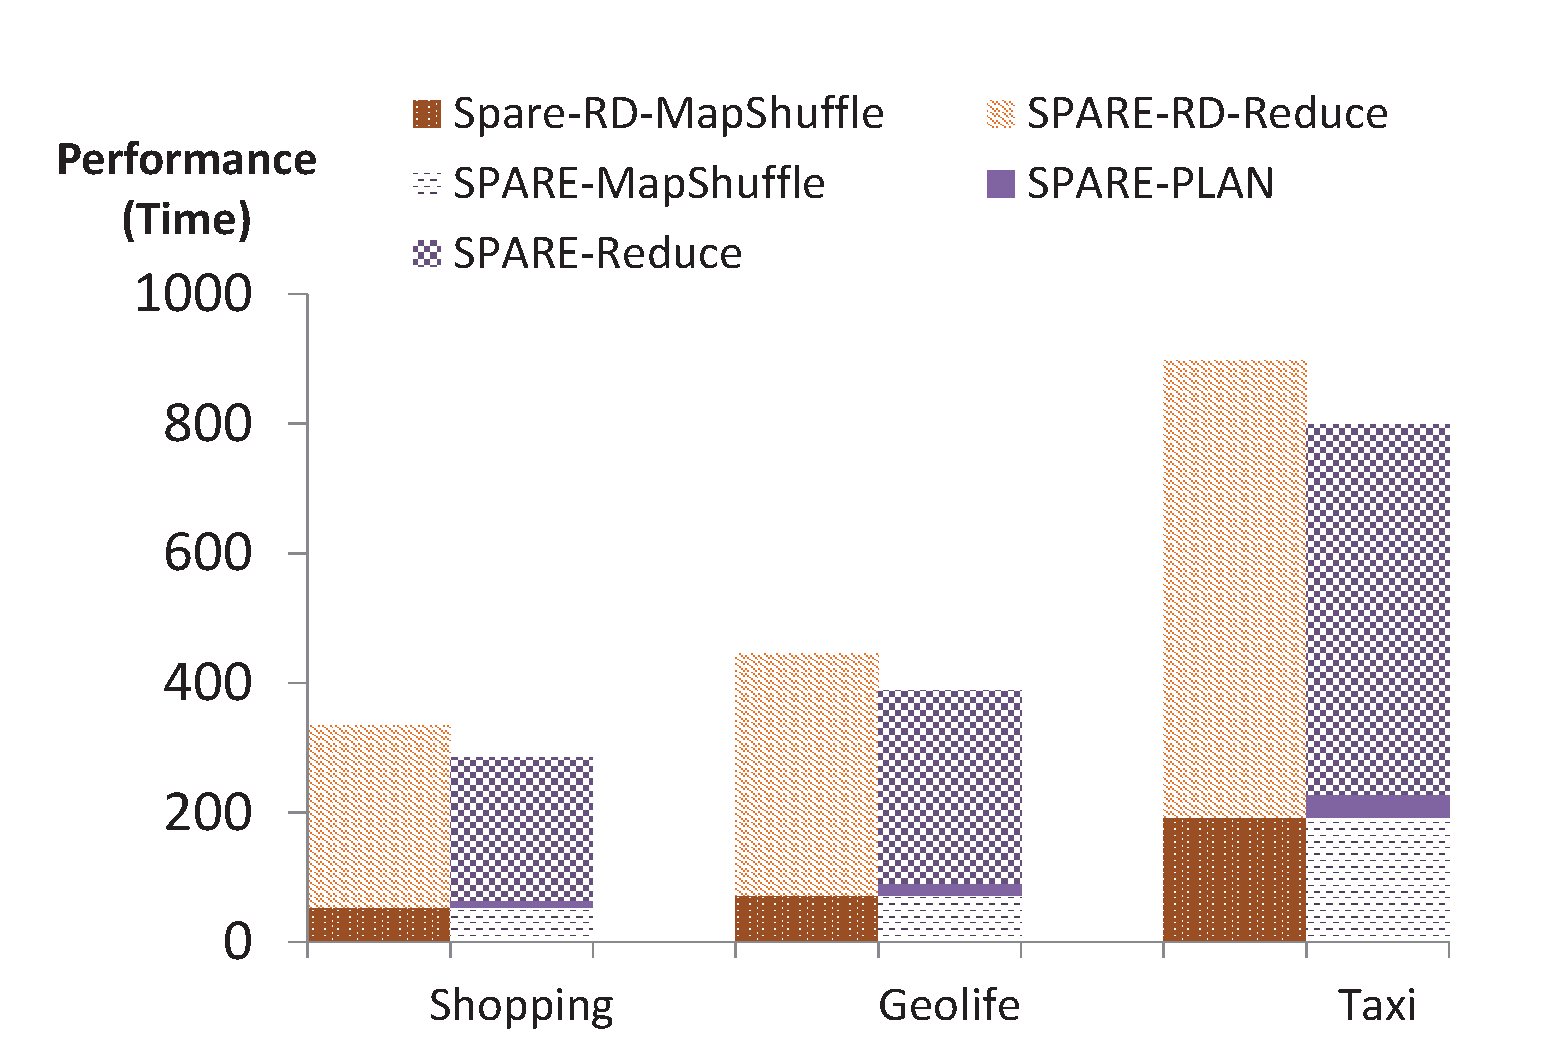
\includegraphics[width=\textwidth]{/exp/spare/detail.eps}
        \caption{Decomposed running time}
    \end{subfigure}
 	 \begin{subfigure}[b]{0.22\textwidth}
        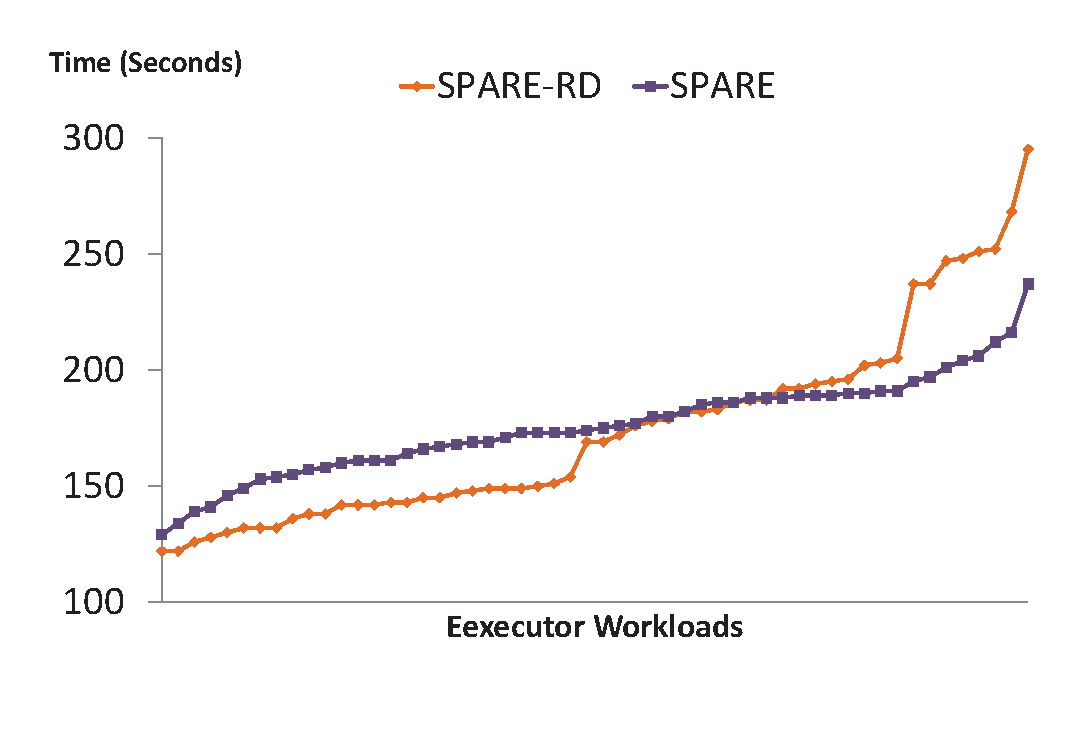
\includegraphics[width=\textwidth]{/exp/spare/wl-shopping.eps}
        \caption{Workload in Shopping}
    \end{subfigure}
    \begin{subfigure}[b]{0.22\textwidth}
        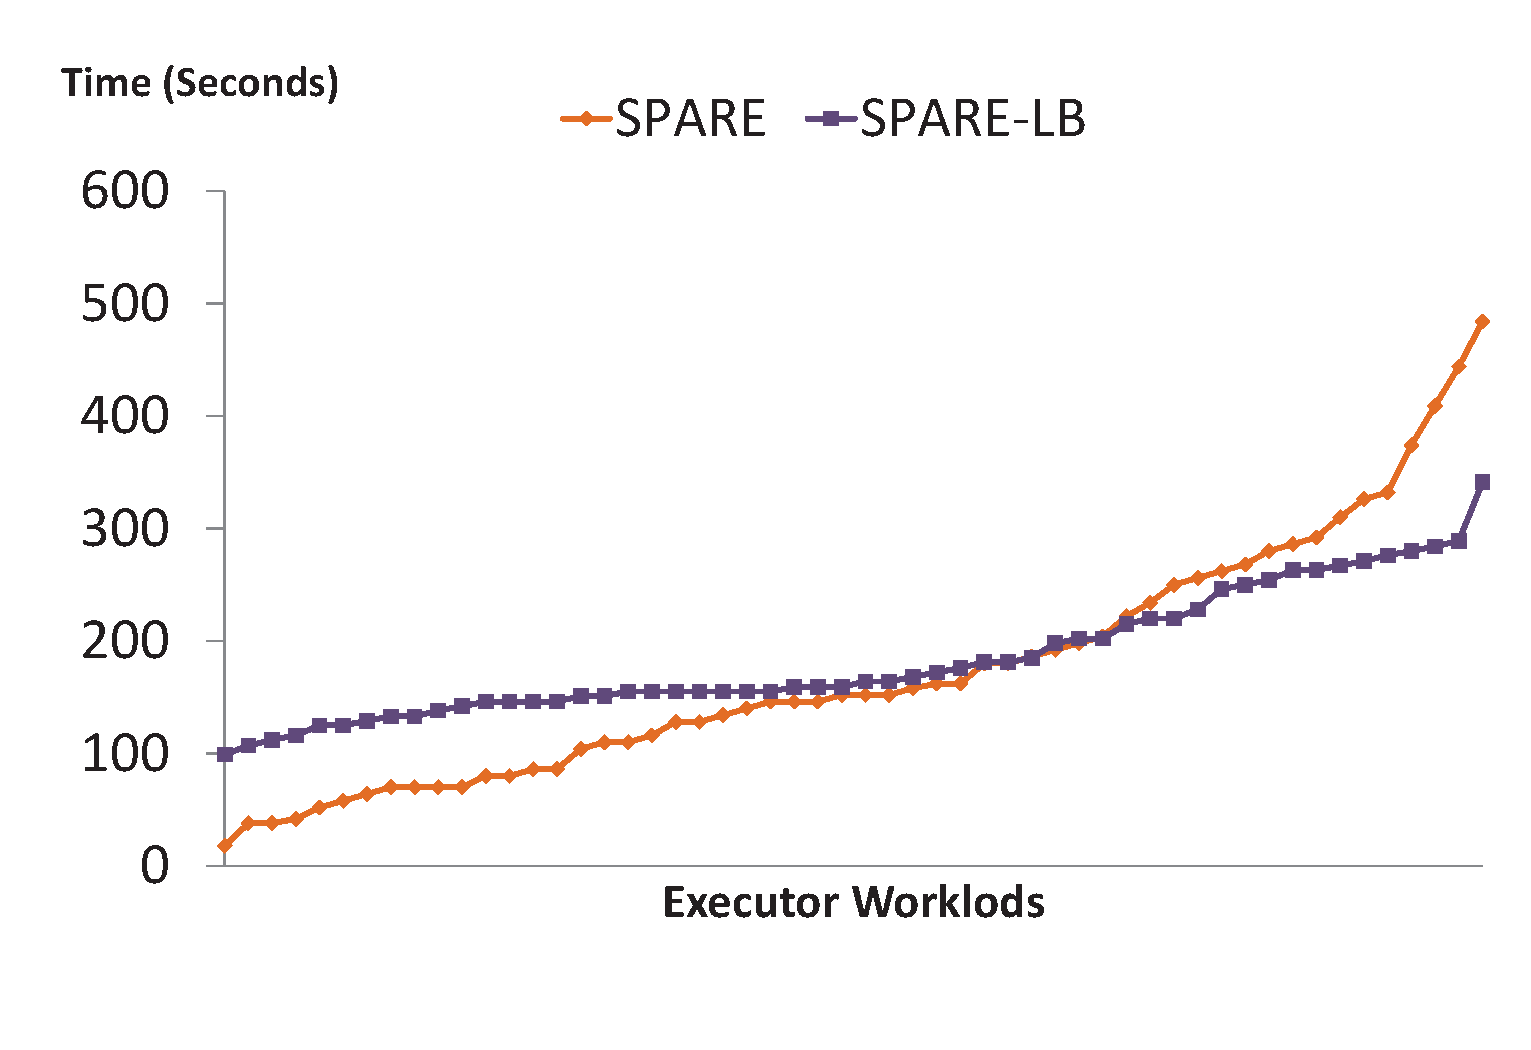
\includegraphics[width=\textwidth]{/exp/spare/wl-geolife.eps}
        \caption{Workload in Geolife}
    \end{subfigure}  
    \begin{subfigure}[b]{0.22\textwidth}
        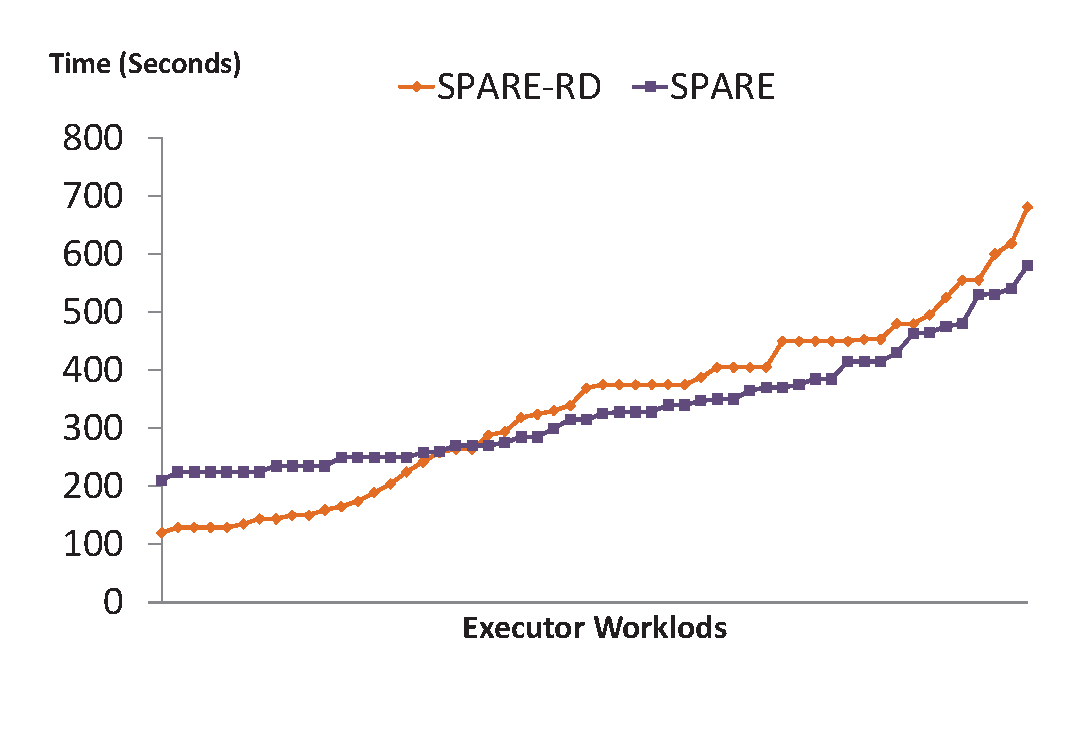
\includegraphics[width=\textwidth]{/exp/spare/wl-taxi.eps}
        \caption{Workload in Taxi}
    \end{subfigure}
\caption{Load balance of SPARE and SPARE-LB}
\label{exp:wl}
\end{figure}

\subsubsection{Load Balance}
To study why SPARE-LB is more efficient,
we analyze the running time of  SPARE and SPARE-LB for 
each map-reduce stage. 
The detail anatomy is shown in Figure~\ref{exp:wl}(a).
We can see that on all three datasets, the reduce phase for both SPARE and SPARE-LB takes the majority time. The overall improvement of SPARE-LB is around 10-13\%
under the default settings. We observe that the map and shuffle time
of SPARE and SPARE-LB are identical, where SPARE-LB spends a very small portion of extra time (4\% of the total time)
in applying the best-fit strategy. The time spent is worthwhile
as in the reduce phase SPARE-LB saves around 20\% of the time. However, since the star sizes in SPARE is almost identical (due to Theorem~2), the best-fit strategy does not win too significantly.

We then look at the workload distribution of SPARE and SPARE-LB on real datasets. We collect the statistics from executors
and report their reduce times in Figure~\ref{exp:wl}. The figure shows that SPARE-LB is able to provide a more balanced task allocation in all three cases. Since SPARE takes random assignment
of stars, it is likely to assign many large stars to the same executor. As we can see the difference between stragglers in
SPARE-LB and SPARE ranges from 60 seconds to 100 seconds. In general cases, SPARE-LB is recommended as it offers more efficiency while takes only a small extra time for planning.

\subsubsection{Scalability}
We then study the scalability of SPARE-LB from two aspects. 
First, we fix the computing power and vary the size of dataset.
We perform a random sample from the tree dataset and the results of SPARE-LB are shown in Figures~\ref{fig:scalability-wl}. As the figures show, SPARE-LB grows almost linearly wrt $|O|$ and $|T|$. This suggests a good scalability. 
Note that, as shown in Figure~\ref{fig:related_work_scalability}, a centralized algorithm runs more than a hundred times slower than SPARE for the same scale of data. This confirms the superiority of our parallel

\begin{figure}[h]
\begin{subfigure}[b]{0.22\textwidth}
\centering
    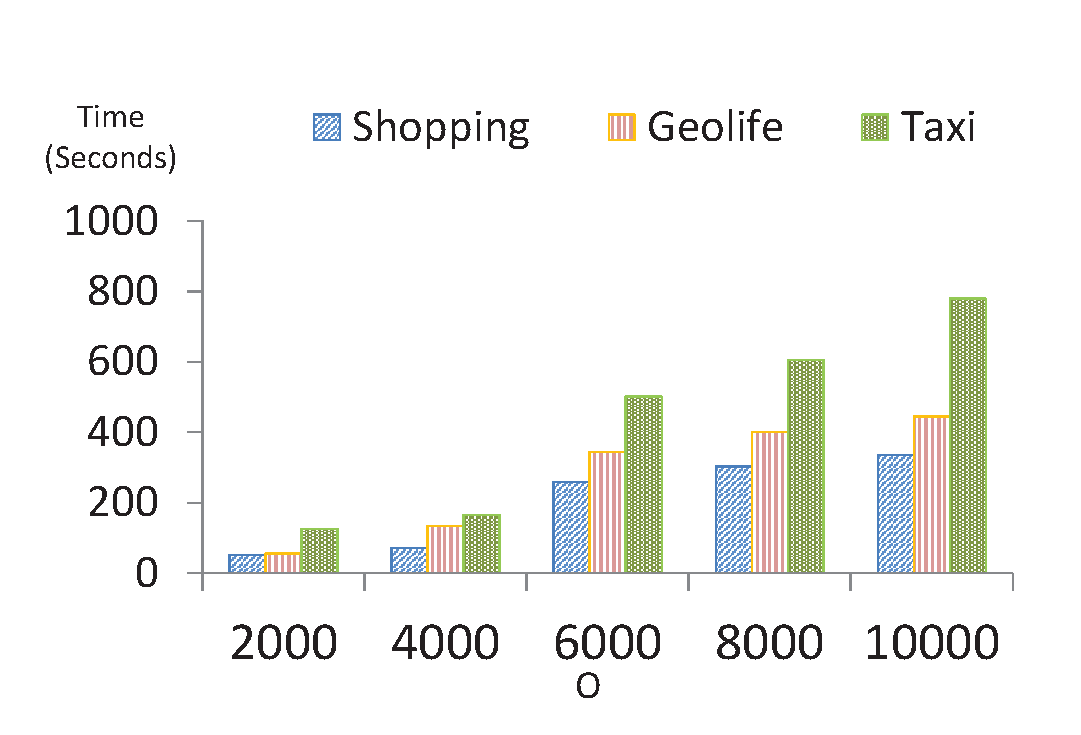
\includegraphics[width=\textwidth]{/exp/spare/scalability-vary-O.eps}
        \caption{Scalability vary $|O|$}
    \end{subfigure}
 	 \begin{subfigure}[b]{0.22\textwidth}
        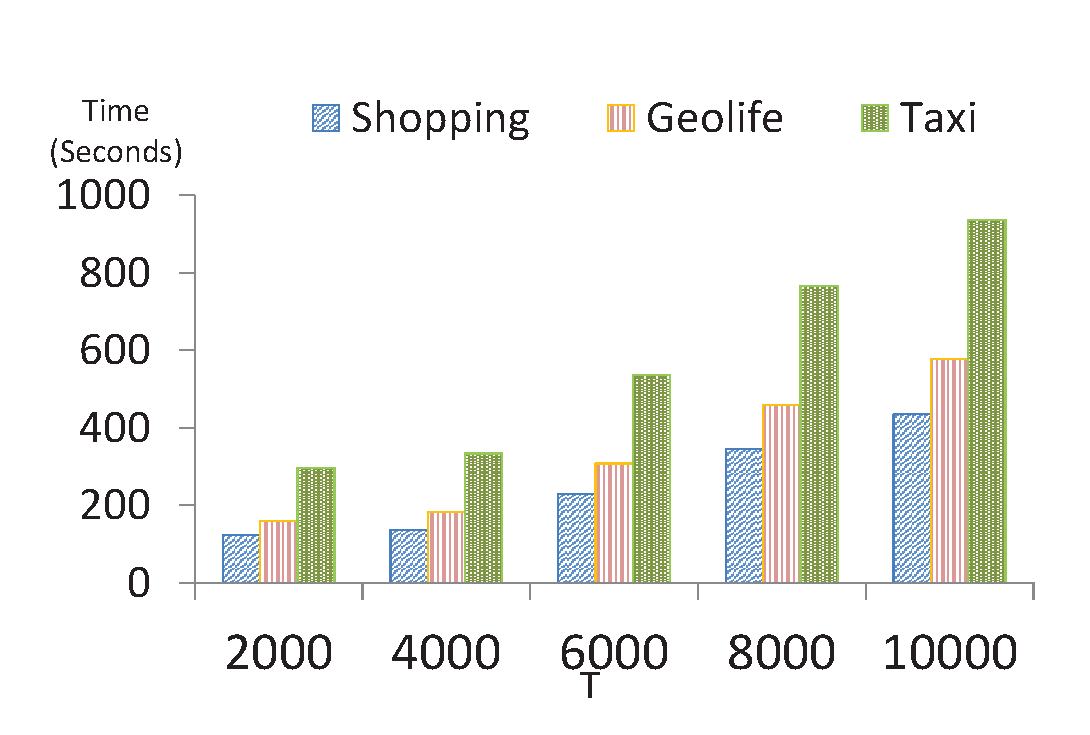
\includegraphics[width=\textwidth]{/exp/spare/scalability-vary-T.eps}
        \caption{Scalability vary $|T|$}
    \end{subfigure}
 \caption{Scalability of SPARE-LB wrt. different data sizes}
 \label{fig:scalability-wl}
\end{figure}

Second, we fix the work load and vary the number of executors.
The result are presented in Figure~\ref{exp:scalability}.
We can see that SPARE achieves good scalability under all three cases. 
For instance, for Taxi dataset, when the executors rises from 10 to 50, 
the performance improves 4.8 times which is almost linear to the increase of executors. Such pattern also holds for the other two datasets. The reason for the good scalablity is that SPARE partitions the trajectories by objects and each partition is perfectly independent. Therefore, when the number of reducers $N << |O|$, SPARE can always speed up by adding more executors.
\begin{figure}[h]
\centering
   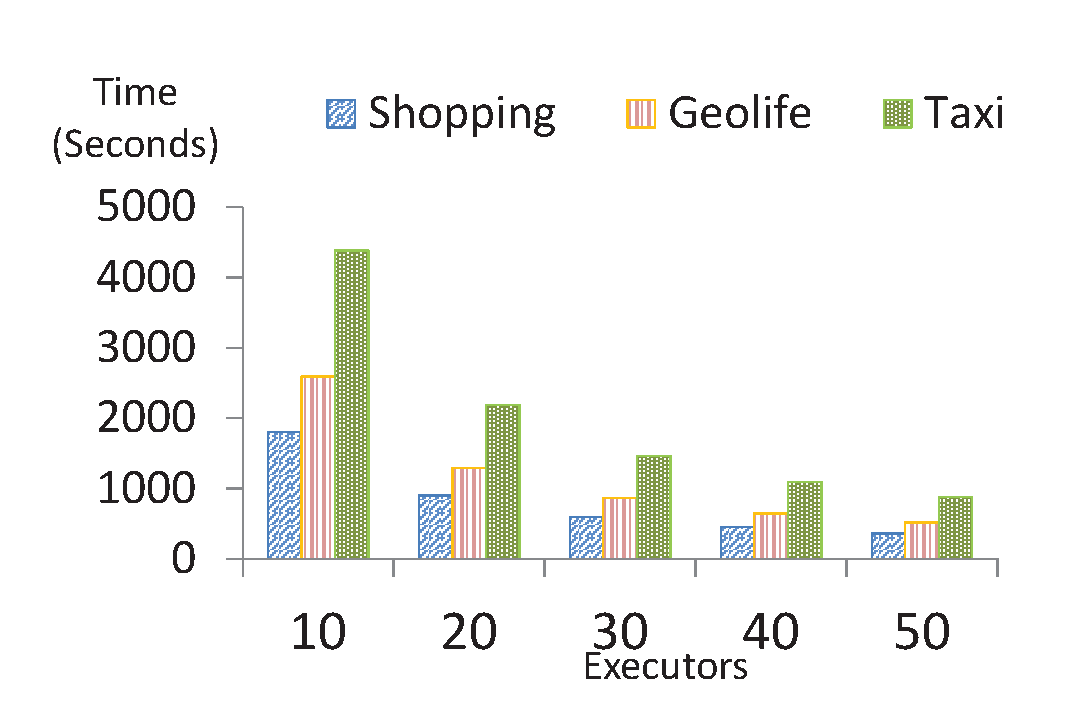
\includegraphics[width=0.3\textwidth]{/exp/spare/scalability.eps}
\caption{Scalability of SPARE-LB vary. $N$.}
\label{exp:scalability}
\end{figure}



